\documentclass{article}
\usepackage[CJKchecksingle,CJKnumber]{xeCJK} %解决中文显示问题
\usepackage{tikz}
\usepackage{pgfplots}
\usepackage{amsmath}
\usepackage{indentfirst}
\usepackage{setspace}
\usepackage{CJKnumb}% 阿拉伯数字转中文数字(用于计数)


\newCJKfontfamily[fs]\fs{FangSong} % 仿宋
\newCJKfontfamily[kai]\kai{KaiTi} % 楷体
\newCJKfontfamily[yh]\yh{Microsoft YaHei}
\setlength{\parindent}{2em} % 设置首行缩进2个字符(只对段落有效)
\setmainfont{Times New Roman} % 设置英文主要字体
\newcounter{x2}% 自定义计数器
\usecounter{x2}
\newcounter{x3}[x2]
\usecounter{x3}
\setcounter{x3}{1}
\newcounter{x4}[x3]
\usecounter{x4}
\setcounter{x4}{1}
\newcounter{x5}[x4]
\usecounter{x5}
\setcounter{x5}{1}
\newcommand{\updateCounter}[2]{\stepcounter{#1}\setcounter{#2}{1}}
\pgfplotsset{compat=1.11}

% \setCJKfamilyfont{kai}{KaiTi} 
% \newcommand*{\kai}{\CJKfamily{kai}}
\newcommand{\TP}[1]{\begin{spacing}{1.4}\par{#1}\end{spacing}}
\newcommand{\TL}[1]{\begin{flushleft}#1\end{flushleft}}
\newcommand{\TR}[1]{\begin{flushright}#1\end{flushright}}
\newcommand{\TC}[1]{\begin{center}#1\end{center}}
\newcommand{\x}[1]{\TL{\fontsize{28pt}{0}\textbf{\kai#1}\\[1.5em] \hrule}}
\newcommand{\xx}[1]{\TL{\fontsize{24pt}{0}\textbf{\yh#1}\\[1.5em]}}
\newcommand{\xxx}[1]{\TL{\fontsize{20pt}{0}\textbf{\yh\CJKnumber{\arabic{x3}}、#1}\\[1.5em]}\updateCounter{x3}{x4}}
\newcommand{\xxxx}[1]{\TL{\fontsize{16pt}{0}\textbf{\yh\arabic{x4}. #1}\\[1.5em]}\updateCounter{x4}{x5}}
\newcommand{\xxxxx}[1]{\TL{\fontsize{12pt}{0}\textbf{\yh(\arabic{x5})  #1}\\[1.5em]}\stepcounter{x5}}
\newcommand{\xxxxxx}[1]{\TL{\fontsize{10pt}{0}\textbf{\yh#1}\\[1.5em]}}
\newcommand{\xs}[1]{\TL{\fontsize{8.5pt}{0}#1\\[1.5em]}}

\begin{document}
	\x{深度学习笔记}
	
	\xxx{深度学习模型}
	
	\def\layersep{3cm}
	
	\xxxx{神经网络示意图}
	\TC{
	\begin{tikzpicture}[shorten >=1pt,->,draw=black!80, node distance=\layersep]
	\tikzstyle{every pin edge}=[<-,shorten <=1pt]
	\tikzstyle{neuron}=[circle,fill=black!25,minimum size=17pt,inner sep=0pt]
	\tikzstyle{input neuron}=[neuron, fill=green!50];
	\tikzstyle{output neuron}=[neuron, fill=red!50];
	\tikzstyle{hidden neuron}=[neuron, fill=blue!50];
	\tikzstyle{annot} = [text width=4em, text centered];
	\tikzstyle{tip} = [minimum height=1.5em];
	
	% Draw the input layer nodes
	\foreach \name / \y in {1,...,4}
	% This is the same as writing \foreach \name / \y in {1/1,2/2,3/3,4/4}
	\node[input neuron, pin=left:Input \#\y] (I-\name) at (0,-\y) {$x_\y$};
	
	% Draw the hidden layer nodes
	\foreach \name / \y in {1,...,5}
	\path[yshift=0.5cm]
	node[hidden neuron] (H-\name) at (\layersep,-\y cm) {};
	
	% Draw the output layer node
	\node[output neuron,pin={[pin edge={->}]right:Output}, right of=H-3] (O) {$y$};
	
	% Connect every node in the input layer with every node in the
	% hidden layer.
	\foreach \source in {1,...,4}
	\foreach \dest in {1,...,5}
	\path (I-\source) edge (H-\dest);
	
	% Connect every node in the hidden layer with the output layer
	\foreach \source in {1,...,5}
	\path (H-\source) edge (O);
	
	% Annotate the layers
	\node[annot,above of=H-1, node distance=1cm] (hl) {Hidden layer};
	\node[annot,left of=hl] {Input layer};
	\node[annot,right of=hl] {Output layer};
	\end{tikzpicture}
	}
	\TC{一个2层的full-connect神经网络\\[2em]}
	
	\TC{
	\begin{tikzpicture}[shorten >=1pt,->,draw=black!80, node distance=\layersep]
	\tikzstyle{neuron}=[circle,fill=black!25,minimum size=20pt,inner sep=0pt]
	\tikzstyle{tip}=[rectangle, minimum size=20pt]
	\tikzstyle{edge}=[<-,shorten <=1pt];
	\tikzstyle{input}=[neuron, fill=blue!40];
	\tikzstyle{op}=[tip, fill=yellow!40];
	\tikzstyle{para}=[tip, fill=green!40];
	\tikzstyle{hidden}=[neuron, fill=red!40];
	\tikzstyle{output}=[neuron, fill=orange!40];
	\tikzstyle{to}=[->,>=stealth,shorten >=1pt,semithick,font=\sffamily\footnotesize];
	
	\node[input] (x1) at (0,-1) {$x_1$};
	\node[input] (x2) at (0,-2) {$x_2$};
	\node[op] (o1) at (\layersep,-1.5) {$+$};
	\node[hidden] (z) at (1.5*\layersep,-1.5) {$z$};
	\node[output] (y) at (2.5*\layersep, -1.5) {$y$};
	\node[para] (b) at (\layersep, -1.25*\layersep) {$b$};
	
	\path (x1) edge node[para,midway,above]{$w_1$} (o1);
	\path (x2) edge node[para,midway,below]{$w_2$} (o1);
	\path (b) edge (o1);
	\path (o1) edge (z);
	\path (z) edge node[op,midway,above]{$\sigma(z)$} (y);
	\end{tikzpicture}
	}
	\TC{$f(x)=wX+b$线性模型 + $\sigma(z)$激活函数\\[2em]}
	
	\xxxx{深度学习基本步骤}
	\begin{figure}[ht]
		\centering
		\includegraphics[scale=0.6]{dl_1.jpg}
		\caption{步骤图(来自李宏毅)}
	\end{figure}
	
	\xxxxx{搭建神经网络}
	\TP{搭建神经网络需要确定神经网络类型、隐藏层的神经元个数、神经网络的层数、初始化参数、选择合适的激励函数和学习率(learning rate)等等。}
	
	\xxxxx{调整参数(learning)}
	\TP{通过梯度下降法,找到使得Cost Function(即$\sum\limits_{i=1}^{m}L_i$)最小的参数;这里需要使用BP算法算出每个参数的梯度值。}
		
	\xxx{技巧}
	
	\xxxx{Backpropagation}
	
	\xxxxx{梯度下降法}
	\TP{\textbf{梯度下降法(gradient descent)}是一个最优化算法,通常也称为最速下降法。梯度下降法的计算过程就是沿梯度下降的方向求解极小值(也可以沿梯度上升方向求解极大值)。常用于机器学习和人工智能当中用来递归性地逼近最小偏差模型。}
	\TP{若定义Cost Function为:$J(w,b)=\sum\limits_{i=1}^m L(y_i,\hat{y}_i)$,则通过梯度下降学习参数的过程为:}
	\TC{\begin{tikzpicture}[shorten >=1pt,->,draw=black!80, node distance=\layersep]
	\tikzstyle{box} = [rectangle,minimum height = 2.5em,rounded corners];
	\tikzstyle{edge1}=[<-,shorten <=1pt];
	\tikzstyle{nimei}=[<-,shorten <=1pt];
	
	\node[box, fill=blue!20] (b1) at (0, -1) {$\displaystyle\nabla{J}=\begin{bmatrix}
		\dfrac{\partial{J}}{\partial{w_1}} \\[1.5em]
		\dfrac{\partial{J}}{\partial{w_2}} \\[1.5em]
		\cdots \\[1.5em]
		\dfrac{\partial{J}}{\partial{w_n}} \\[1.5em]
		\dfrac{\partial{J}}{\partial{b}}
		\end{bmatrix}$};
	\node[box, fill=orange!20] (b2) at(1.6*\layersep, -1) {$\displaystyle\begin{bmatrix}
		w_1 \\
		w_2 \\
		\cdots \\
		w_n \\
		b\end{bmatrix}=\begin{bmatrix}
		w_1 \\
		w_2 \\
		\cdots \\
		w_n \\
		b\end{bmatrix}-\alpha*\nabla{J}$};
	\node[box, fill=green!20] (b3) at (3*\layersep, -1){$\nabla{J}<\delta\simeq 0?$};
	\node[box, fill=green!20, below of=b3](b4) {$\displaystyle\begin{bmatrix}
		w_1 \\
		w_2 \\
		\cdots \\
		w_n \\
		b\end{bmatrix}$};
	
	\path (b1) edge (b2);
	\path (b2) edge (b3);
	\path (b3) edge[->, bend right=45] node[midway, above]{No} (b1);
	\path (b3) edge[->] node[right, midway]{Yes} (b4);
	\node[box, below of=b2, node distance=2cm] {更新参数(梯度下降逼近极小值点)};
	\node[box, below of=b1] {计算梯度};
	\node[box, below of=b4, node distance=2cm] {最终参数(使得Cost最小)};
	
	\end{tikzpicture}}
	\TC{梯度下降法简易流程图\\[2em]}
	
	\xxxxx{反向传播}
	\TP{反向传播,顾名思义就是沿着与神经网络前进相反的方向进行数据传播,可以理解为神经元的反馈;BP可用于计算神经网络中每层参数的梯度值,利用的是求导链式法则;}
	\TP{可以这么理解,假设神经网络中相邻的两层$H_i,H_{i+1}$,$H_i$作为$H_{i+1}$的input,那么相对而言output就是$H_{i+1}$,因此两者间有线性关系;}
	\TC{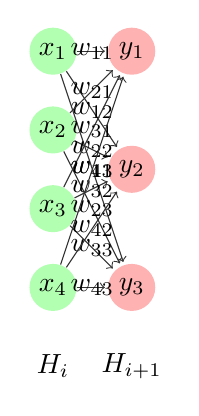
\begin{tikzpicture}[shorten >=1pt,->,draw=black!80, node distance=\layersep]
	\tikzstyle{neuron}=[circle,fill=black!25,minimum size=17pt,inner sep=0pt];
	
	\foreach \name in {1,...,4}
	\node[neuron, fill=green!30] (A\name) at (0, -\name) {$x_{\name}$};
	
	\foreach \name in {1,...,3}
	\node[neuron, fill=red!30] (B\name) at (\layersep, -\name*1.5 + 0.5) {$y_{\name}$};
	
	\foreach \nx in {1,...,4}
	\foreach \ny in {1,...,3}
	\path (A\nx) edge[->] node[midway,midway]{$w_{\nx\ny}$} (B\ny);
	\node[rectangle,below of=A4,node distance=1cm]{$H_i$};
	\node[rectangle,below of=B3,node distance=1cm]{$H_{i+1}$};
	
	\end{tikzpicture}}
	\TP{因此,计算相邻的参数梯度即为其对应的参数$w_{ij}$,如:$\dfrac{\partial{y_3}}{\partial{x_4}}=w_{43}$;然后依据链式法则,即可算出从最后的Cost Function到任意一层的任一参数的偏微分$\dfrac{\partial{J}}{\partial{w_{ij}}}$,所谓的反向传播在这里就是从最后一层向前进行连续的链式求导求出各参数的偏微分!}
	\begin{figure}[ht]
		\centering
		\includegraphics[scale=0.6]{dl_2.png}
		\caption{反向链式求导(来自李宏毅)}
	\end{figure}
	\TP{如果$H_i,H_{i+1}$并非直接的相邻关系,中间多了一个激励函数$\sigma(z)$作为输出的话,那么根据链式求导法则再多求一次就好了!(见上图)}
	
	\xxxx{激励函数(activation function)}
	\xxxxx{Sigmoid函数}
	\TP{Sigmoid定义为:$\sigma(z)=\dfrac{1}{1+e^{-z}}$,所以可以看出其输出值在[0,1]之间,因此比较适合来表示概率!但是其有一个比较明显的缺点,从其函数图像可以看出两端的值比较『缓和』,因此梯度接近于0,不利于learning;此外,其图像并非中心对称,而且e的指数幂计算起来比较耗时!}
	\begin{figure}[ht]
		\centering
	\begin{tikzpicture}
	\begin{axis}[width=12cm,height=8cm]
	\addplot[blue,thick,domain=-10:10,samples=200,variable=z]
	{1/(1+exp(-z))};
	\end{axis}
	\end{tikzpicture}
	\caption{Sigmoid函数-$\sigma(z)=\dfrac{1}{1+e^{-z}}$}
	\end{figure}
	\xxxxx{ReLU}
	\TP{Rectified Linear Unit,简称为ReLU,是目前最常用的激励函数之一;其函数形式为$f(x)=max(0,x)$,因此可以看出其左半部分($x<0$)是一个常数0,右半部分是一个一元线性函数$y=x$;}
	\begin{figure}[ht]
		\centering
		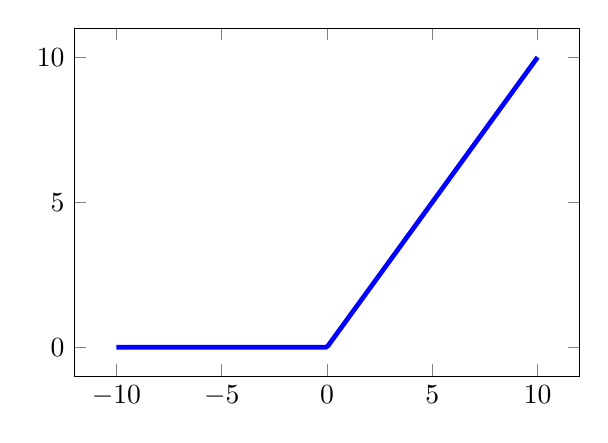
\begin{tikzpicture}
		\begin{axis}[width=8cm,height=6cm]
		\addplot[blue,line width=0.06cm,domain=-10:10,samples=200,variable=x]
		{max(0,x)};
		\end{axis}
		\end{tikzpicture}
		\caption{ReLU-$f(x)=max(0,x)$}
	\end{figure}
	\TP{这样设计的好处有:(1)便于计算(线性);(2)解决梯度消失(Vanishing gradient)的问题;(3)除去负值?}
	\xxxxx{Leaky ReLU}
	\TP{为了弥补ReLU左半部分的不足(小于0会使神经元被『抛弃』,即不影响后续神经元),Leaky ReLU在左半部分做了小小的修正,在左半部分改为一个斜率很小的线性函数,如:$max(0.1x,x)$;}
	\begin{figure}[ht]
		\centering
		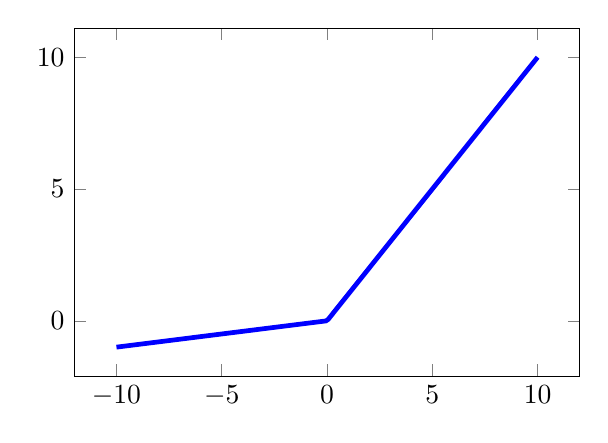
\begin{tikzpicture}
		\begin{axis}[width=8cm,height=6cm]
		\addplot[blue,line width=0.06cm,domain=-10:10,samples=200,variable=x]
		{max(0.1*x,x)};
		\end{axis}
		\end{tikzpicture}
		\caption{Leaky ReLU-$f(x)=max(0.1x,x)$}
	\end{figure}
	\xxxxx{ELU}
	\TP{Exponential Linear Units (ELU),跟Leaky ReLU的修改不同,ELU把左半部分修改为一个非线性的函数——即$f(x)=\begin{cases}\alpha*(e^x-1), &x<0 \\ x, &x\ge 0\end{cases}$;}
	\begin{figure}[ht]
		\centering
		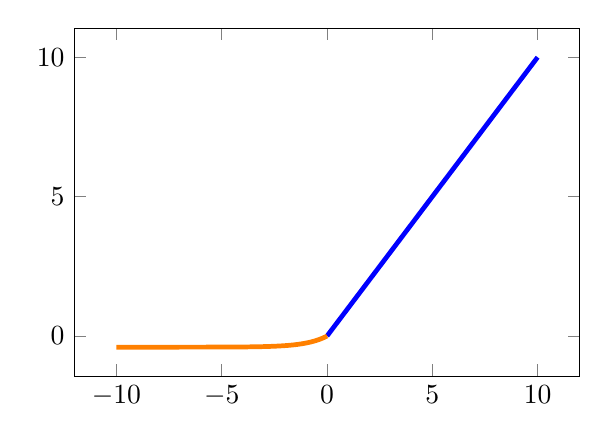
\begin{tikzpicture}
		\begin{axis}[width=8cm,height=6cm]
		\addplot[blue,line width=0.06cm,domain=0:10,samples=200,variable=x]
		{x};
		\addplot[orange,line width=0.06cm,domain=-10:0,samples=200,variable=x]
		{0.4*(e^x-1)};
		\end{axis}
		\end{tikzpicture}
		\caption{ELU-$\alpha=0.4$}
	\end{figure}
	\xxxxx{maxout}
	\TP{maxout,顾名思义就是输出最大值,一般将$k$个神经元的输出值进行比较选出其中最大的输出值,即:$max(w_1x+b_1,\cdots,w_kx+b_k)$;关键是在于比较的神经元的数量$k$以及它们之间的位置如何选择,一般是选取相邻的神经元?}
	\begin{figure}[ht]
		\centering
		\includegraphics[scale=0.6]{dl_3.jpg}
		\caption{maxout训练过程(来自李宏毅)}
	\end{figure}
	
	\xxxx{Dropout}
	\TP{Dropout的大致思想是在learning过程中对每一层神经层中神经元以概率$p$进行『舍弃』(注意:这里的舍弃并非真正舍去,而是仅仅在这一次迭代更新中将这些神经元不加入计算行列而已,即每次迭代更新参数过程中都进行一次随机dropout,因此每次『舍去』的神经元都不一样);至于为何要这么做,大概是因为以下几个原因:}
	\begin{enumerate}
		\item 减少计算量:因为每次learning的过程中,减去了很多神经元,所以神经网络的复杂度大大降低,计算量肯定是减少的;(精度能保证吗?)
		\begin{figure}[ht]
			\centering
			\includegraphics[scale=0.6]{dl_4.jpg}
			\caption{dropout训练过程(来自李宏毅)}
		\end{figure}
		\item 集成(ensemble):因为每次的迭代过程『舍去』的神经元都不一样,所以每次迭代的神经网络的构造肯定是不同的,因此就相当于对多个神经网络同时进行learning,也就是所谓的ensemble learning(?);
		\begin{figure}[ht]
			\centering
			\includegraphics[scale=0.6]{dl_6.jpg}
			\caption{集成化(来自李宏毅)}
		\end{figure}
		\begin{figure}[ht]
			\centering
			\includegraphics[scale=0.6]{dl_5.jpg}
			\caption{ensemble learning示意图(来自李宏毅)}
		\end{figure}
		\item 防止过拟合:
	\end{enumerate}
	\TP{需要注意的是,在使用了Dropout后,在之后的testing过程中需对所有的参数乘上$1-p$!(为何?)}
	
	\xxxx{Regularization(正则化)}
	\TP{正则化就是通过调整代价函数(Cost Function)来防止参数产生过拟合的现象,主要方式为:$J'(w)=J(w)+\lambda g(w)$,其中$g(w)$是关于所有参数的约束函数,$\lambda$为一个常数;常用的约束函数有$L^1 (\|w\|_1)$和$L^2 (\|w\|_2)$等;因此在梯度下降过程中要使用$\dfrac{\partial{J'}}{\partial{w}}$来代替原来的$\dfrac{\partial{J}}{\partial{w}}$;}
	
	\xxxx{mini-batch}
	\TP{所谓的batch,就是一次处理的数据的规模,用于学习过程中对损失函数的更新方式;mini-batch就是将所有数据划分为若干个batch,然后每次用一个batch的数据更新损失函数,然后用梯度下降更新所有参数;}
	
	\xxx{卷积神经网络}
	\xxxx{卷积}
	\xxxxx{概念}
	\TP{以前只知道图像中有个卷积的运算,而且很常用,后来没想到在考研复习的时候发现概率论也有卷积运算,我想图像中的离散卷积运算应该是从连续的卷积运算演化过来的吧。连续卷积运算定义为:}
	\TC{$s(t)=\displaystyle\int x(a)w(t-a)da=(x*w)(t)$}
	\TP{一般使用$*$符号作为卷积符号。通常,$w$被称作核函数(kernel function)。}
	\TP{单通道的图像数据可以看做一个二维的数据,图像中卷积的操作形式如下:}
	\TC{$s(i,j)=(I*K)(i,j)=\displaystyle\sum_m\sum_n I(i-m,j-n)*K(m,n)$}
	\TP{与卷积很相近的一种运算叫做相关(correlation)运算($\otimes$),可以这么定义:}
	\TC{$s(i,j)=(I\otimes K)(i,j)=\displaystyle\sum_m\sum_n I(i+m,j+n)\otimes K(m,n)$}
	\TP{但是在实际运用过程中,这两种操作都叫做『卷积』?(deeplearning book一书是这么说的)}
	\xxxxx{作用}
	\TP{为何要在神经网络中使用卷积运算?大概是『参数共享』使每层的参数相比全连接(full-connect)时大大减少,每层的参数仅有核函数的大小。但是很明显,并不是所有的神经网络都能使用卷积操作。对于图像而言,每个核函数就像是一个局部特征检测器,检测一定的与位置无关的特征。}
	\xxxx{池化(pooling)}
	\TP{所谓的池化就是对输入层相邻的一定数据进行筛选,最常用的就是最大池化(max pooling);所谓的最大池化就是选择输入层一定邻域内最大的数据作为输出(有点像maxout?)。}
	\begin{figure}[ht]
		\centering
		\includegraphics[scale=0.8]{dl_7.jpg}
		\caption{max pooling示意图(来自dl-book)}
	\end{figure}
	\TP{池化后的输出具有近似的平移不变性,即少量的位移不会影响大多数的输出结果,这有利于局部特征的检测。}
	
	
\end{document}